\documentclass[12pt,letterpaper]{article}
\usepackage{natbib}

%Packages
% \usepackage{textcomp}
% \usepackage{latexsym}
% \usepackage{url}
% \usepackage{amssymb}
% \usepackage{amsmath}
% \usepackage{mathtools}
% \usepackage{bm}
% \usepackage{array}
% \usepackage[version=3]{mhchem}
% \usepackage{ifthen}
% \usepackage{amsthm}
% \usepackage{amstext}
% \usepackage{enumerate}
% \usepackage{dcolumn}

\usepackage{epsfig}
\usepackage{graphicx}
\usepackage{caption}
\usepackage{hyperref}
\usepackage{lineno}
\usepackage{pdflscape}
\usepackage{mathtools}
\usepackage[osf]{mathpazo}
\usepackage{fullpage}
\usepackage{float}
\usepackage{xr} %linking to supplementaries
\externaldocument{supplementaries}

\pagenumbering{arabic}


%---------------------------------------------
%
%       START
%
%---------------------------------------------

\begin{document}
%Running head
\begin{flushright}
Version dated: \today
\end{flushright}

\bigskip
\bigskip
\begin{center}

\noindent{\Large \bf The what, how and why of trait-based analyses in ecology}
\bigskip

\noindent {\normalsize \sc
Thomas Guillerme$^{1,*}$, 
Pedro Cardoso$^{2,3}$,
Carlos P. Carmona$^{4}$,
Maria Wagner J\o rgensen$^{5}$,
Stefano Mammola$^{3,6,7}$,
Thomas J. Matthews$^{5,8}$}\\
\noindent {\small \it 
$^1$School of Biosciences, The University of Sheffield, Sheffield, S10 2TN, United Kingdom.\\
$^2$CE3C—Centre for Ecology, Evolution and Environmental Changes, CHANGE – Global Change and Sustainability Institute, Faculty of Sciences, University of Lisbon, Lisbon, Portugal\\
$^3$Laboratory for Integrative Biodiversity Research (LIBRe), Finnish Museum of Natural History (Luomus), University of Helsinki, Helsinki, Finland\\
$^4$Institute of Ecology and Earth Sciences, University of Tartu, Tartu, Estonia\\
$^5$School of Geography, Earth and Environmental Sciences and Birmingham Institute of Forest Research, University of Birmingham, Birmingham B15 2TT, UK\\
$^6$Molecular Ecology Group (MEG), Water Research Institute, National Research Council (CNR-IRSA), Verbania Pallanza, Italy\\
$^7$National Biodiversity Future Center, Piazza Marina 61, 90133 Palermo, Italy\\
$^8$Centre for Ecology, Evolution and Environmental Changes/Azorean Biodiversity Group / CHANGE – Global Change and Sustainability Institute and Universidade dos Açores – Faculty of Agricultural Sciences and Environment; PT-9700-042, Angra do Hero\'ismo, A\c ores, Portugal.\\}

\end{center}
\bigskip
\noindent{*\bf Corresponding author.} \textit{t.guillerme@sheffield.ac.uk}\\ 
\vspace{1in}

%Line numbering
\modulolinenumbers[1]
\linenumbers

%---------------------------------------------
%
%       ABSTRACT
%
%---------------------------------------------


\section{Supplementary materials}

\subsection{Supplementary results}

\begin{figure}[!htbp]
\centering
   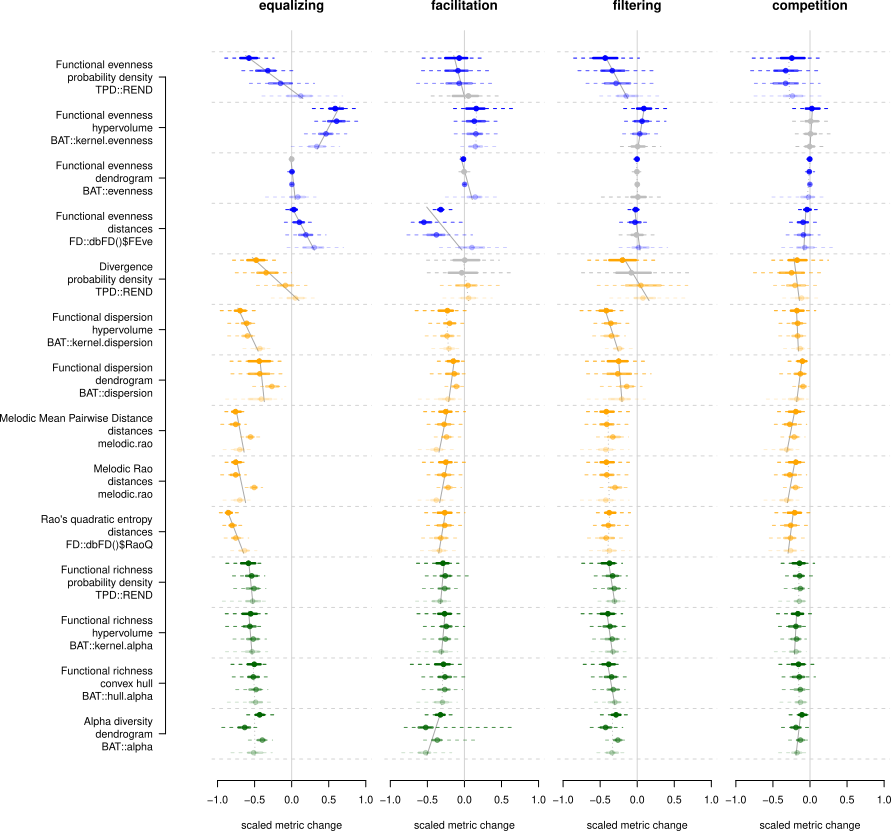
\includegraphics[width=0.8\textwidth]{Figures/results_per_metric_per_stressor_2d.pdf}
\caption{\scriptsize{\textbf{Simulation results for 2 dimensions:} the y axes represent the different metrics tested (sorted by categories).
The different columns represent the different stressors. The x-axes represent the metric values centred on the random changes and scaled by the maximum value for each metric between the four stressors.
Negative and positive values signify a decrease/increase in the metric score.
The dots represent the median metric value, the full line their 50\% confidence interval (CI) and the dashed line their 95\% CI.
The colours are here to visually separate the metrics by categories (blue = regularity, yellow = divergence, green = richness); the colour gradient within each row corresponds to a removal of respectively 80\%, 60\%, 40\% and 20\% of the data (from top to bottom).
The grey line plots represent distributions of metric scores not clearly distinguishable from the random metric scores (paired t-test p value > 0.05).
Grey lines in the background across the distributions of different removal amounts represent the fitted linear model centred and scaled metric score $\sim$ amount of data removed and the value displayed is the adjusted $R^2$ from each of these models.
Dashed thin grey lines represent non-significant models (p value of slope or/and intercept $> 0.05$).
}}
\label{Fig:simulation_results}
\end{figure}
\bigskip


\begin{figure}[!htbp]
\centering
   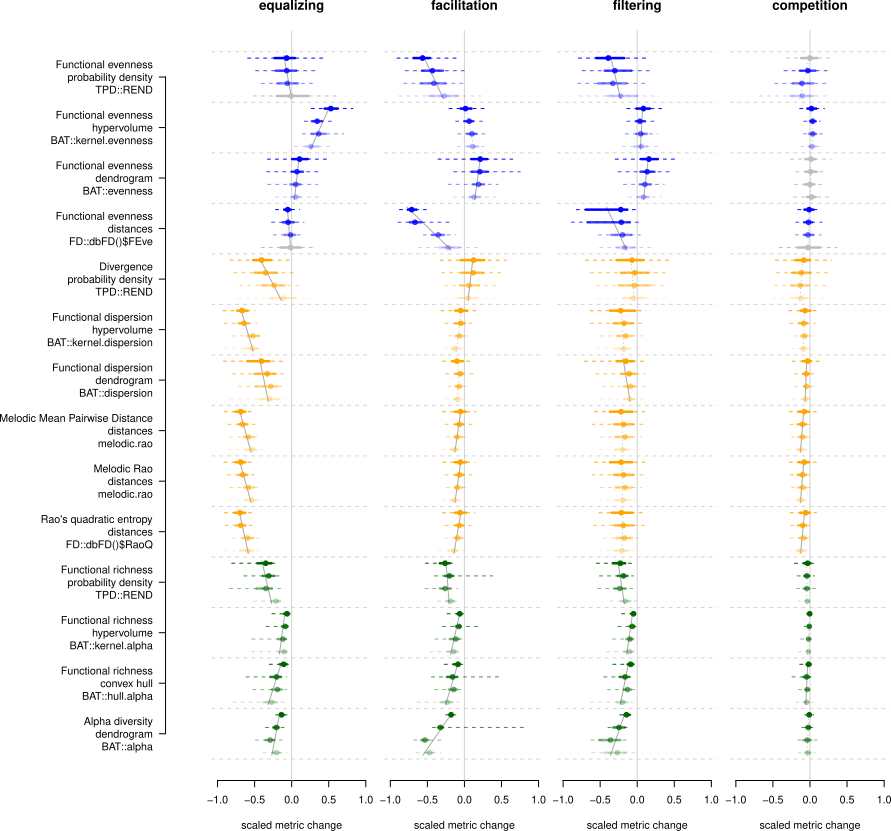
\includegraphics[width=0.8\textwidth]{Figures/results_per_metric_per_stressor_8d.pdf}
\caption{\scriptsize{\textbf{Simulation results for 8 dimensions:} the y axes represent the different metrics tested (sorted by categories).
The different columns represent the different stressors. The x-axes represent the metric values centred on the random changes and scaled by the maximum value for each metric between the four stressors.
Negative and positive values signify a decrease/increase in the metric score.
The dots represent the median metric value, the full line their 50\% confidence interval (CI) and the dashed line their 95\% CI.
The colours are here to visually separate the metrics by categories (blue = regularity, yellow = divergence, green = richness); the colour gradient within each row corresponds to a removal of respectively 80\%, 60\%, 40\% and 20\% of the data (from top to bottom).
The grey line plots represent distributions of metric scores not clearly distinguishable from the random metric scores (paired t-test p value > 0.05).
Grey lines in the background across the distributions of different removal amounts represent the fitted linear model centred and scaled metric score $\sim$ amount of data removed and the value displayed is the adjusted $R^2$ from each of these models.
Dashed thin grey lines represent non-significant models (p value of slope or/and intercept $> 0.05$).
}}
\label{Fig:simulation_results}
\end{figure}
\bigskip


\bibliographystyle{sysbio}
\bibliography{references}


\end{document}